\documentclass[12pt]{beamer}
%
% Choose how your presentation looks.
%
% For more themes, color themes and font themes, see:
% http://deic.uab.es/~iblanes/beamer_gallery/index_by_theme.html
%
\mode<presentation>
{
  \usetheme{default}      % or try Darmstadt, Madrid, Warsaw, ...
  \usecolortheme{default} % or try albatross, beaver, crane, ...
  \usefonttheme{structuresmallcapsserif}  % or try serif, structurebold, ...
  \setbeamertemplate{navigation symbols}{}
  \setbeamertemplate{caption}[numbered]
} 

\usepackage[english]{babel}
\usepackage[utf8]{inputenc}
% \usepackage{graphicx}
\usepackage{verbatim}
\usepackage{multicol}

\title{Title TBA}
\author{Bryant Benzant-Ortiz}
\date{\today}

\begin{document}

\begin{frame}
  \titlepage
\end{frame}

\begin{frame}{Target Specs}
	\begin{itemize}
		\item \textbf{Genre:} Massive Multiplayer Online + Platformer + Sandbox (Open World)
		\item \textbf{Target Age:} Teen
		\item \textbf{Target Platform:} PC (iOS \& Android [as a native app] is a possibility)
	\end{itemize}
\end{frame}

\begin{frame}{Story}
	The player will create a new character by choosing either an angel or devil (demon) and customize his or her body. After that, they will have to pass the final exam before they graduate from middle school and then move on to high school on Earth. They will pack up their items and ship them to their new home at a certain location of the Earth. Now the question: why are they living on Earth? Because there are monsters scattered around the Earth causing trouble and it's up to the angels and devils to work together and stop them at their will while they survive in the common world.
\end{frame}

\begin{frame}{Game Features}
	\begin{itemize}
		\item Meet new angels and devils from around the world
		\item Customize your character with tons of clothing from popular brands
		%\item 
	\end{itemize}
\end{frame}

\begin{frame}{Marketing Scheme}
	\begin{itemize}
		\item Add items from popular brands (e.g., L.L. Bean, The North Face, Coca-Cola)
		\item Players will have a smartphone to chat and they can recommend some items to use and buy in real life (as a way of personal selling)
		%\item 
	\end{itemize}
\end{frame}

\begin{frame}{Game Summary}
	The story begins with the player taking place at the final physical exam--this is the tutorial of the game that teaches player how to play--which takes place before the graduation ceremony. The player will move around, jump on platforms and obstacles, and have to ability to fight. They will also have to press buttons in a sequence to create combos (i.e., Street Fighter). The camera view is a scrolling camera. Players will receive money, food, and a home to stay when they arrive on Earth. They will, however, have to study at high school, work at a part-time job, and fight enemies. The players even have a meter for hunger.
\end{frame}

\begin{frame}{Game Summary (cont.)}
	The environment is basically zones, each that is from a certain country from around the world, that contain three stages, each of them with an airport, a mall, and a residential area with a school included. The stages are basically passages that connect from one non-enemy place to another. Players can also change their place to live and attendance at school if they unlock a zone. There will be eight zones for now (every version update will have eight new zones), six of them are zones that players will stay at and the other two zones are considered to be final bosses (it is not the end of the game, as this is an MMO(RPG), as the game will update).
\end{frame}

\begin{frame}{Game Summary (cont.)}
	\begin{center}
		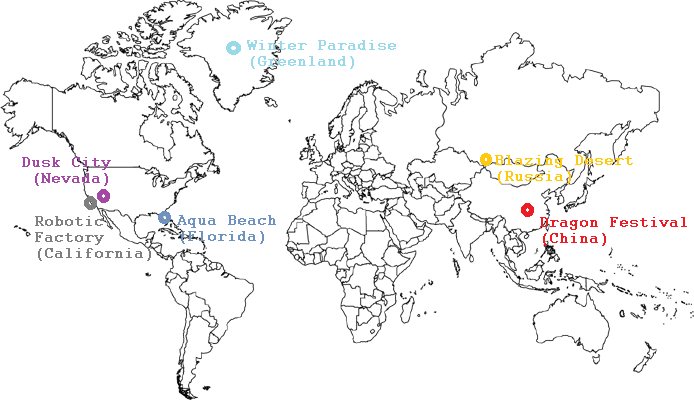
\includegraphics[width=4in]{WorldMapV1}
	\end{center}
	Players can meet other players via battle or at non-enemy places such as coffee shops and malls. They can also go to shops together, play games at arcades, and many real-life hobbies.
\end{frame}

\begin{frame}{Gameplay}
	Players can defeat enemies and gain various items such as money, health, and so on. Every time players defeat enemies, they gain experience points. When players level up by 1, they get to play a bonus stage; the gameplay depends on how many players, or friends in a team, leveled up. \newline

	Players will have to make good choices on what to do when fighting and what to shop for when heading out. For instance, if someone were to buy a High Sierra backpack that has a rain cover, but has a lot of room to put valuables in there, then the player's speed will decrease when running or walking, but will protect items from getting destroyed (valuables will be very sensitive to rain). Otherwise, if someone were to buy an L.L. Bean bag, the player's speed will remain the same or decrease, due to it's space being low and it won't protect valuables in there.
\end{frame}

\begin{frame}{Monetization}
	Players will have a set of currencies when they defeat monsters and buy items; whatever zone (or country) you are at, the currency must belong to the country in order to make a purchase. The upside to that is there is a currency exchange center provided at each mall of the zone.
\end{frame}

\end{document}
